\subsection{Backend -- Middleware layer}
This section presents the services that make up the middleware.

Before seeing every service in detail, it is useful to have an overview to the
organization of those components.

\begin{figure}[H]
  \centering
  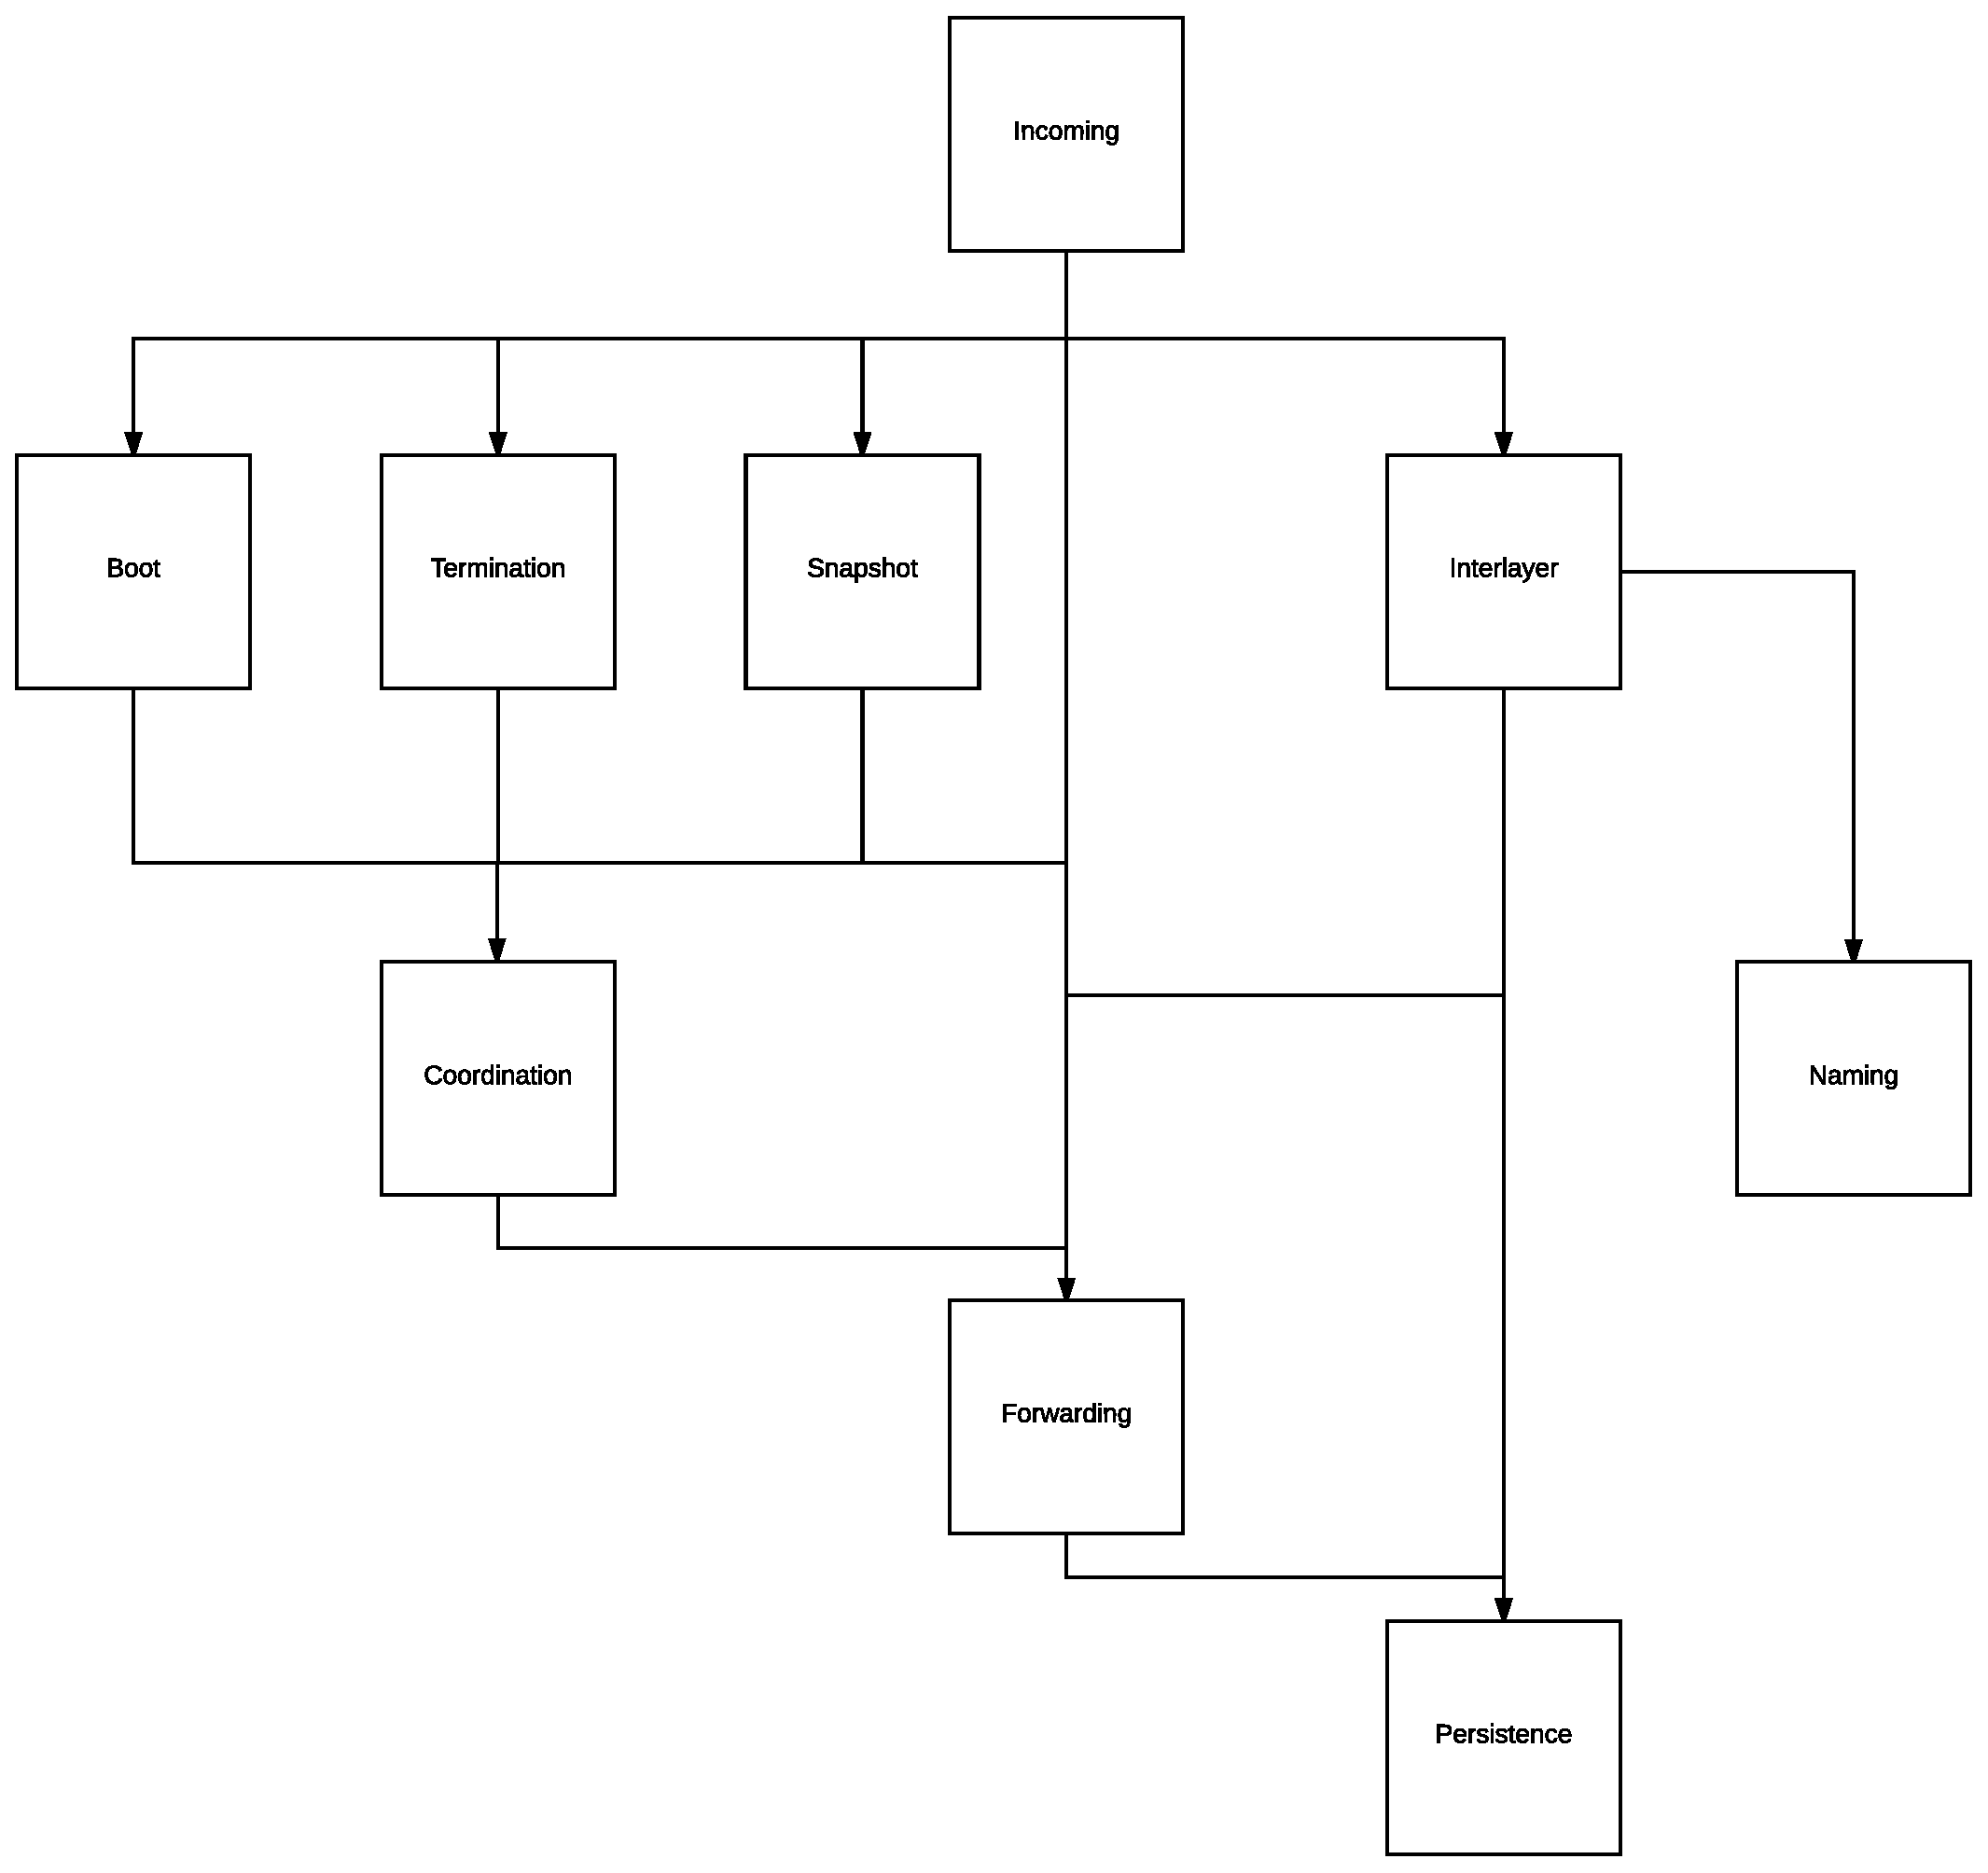
\includegraphics[width=\columnwidth]{images/solution/mw/overview.eps}
  \caption{Middleware architecture overview}
  \label{fig:mw-arch-over}
\end{figure} % TODO: Remove naming package

\begin{itemize}
  \item \texttt{naming}: service that provides a correspondence between logic
    names and their actual location;
  \item \texttt{forwarding}: service that represents the abstraction through
    which it is possible to deliver messages to other middleware nodes;
  \item \texttt{incoming}: service that is responsible of handling messages
    coming from other middleware nodes;
  \item \texttt{interlayer}: service that represents the interface between
    the application and middleware layers;
  \item \texttt{boot}: service that is responsible to start the system neatly;
  \item \texttt{termination}: service that shut downs the node and the system
    gracefully;
  \item \texttt{snapshot}: service that takes consistent views of the node and
    the system;
  \item \texttt{coordination}: service that coordinates the interaction among
    the nodes of the system;
  \item \texttt{persistence}: service that provides a set of utilities to
    store data in a persistent way.
\end{itemize}

\subsubsection{Naming service}

\subsubsection{Forwarding service}
The Forwarding service has to deliver messages to other nodes. This component
is very simple, since it just has an interface (\texttt{MQProxy}) and its
implementation, \texttt{RabbitSender}.

Basically, a \texttt{RabbitSender} takes a message as input and guarantees to
send it to the intended recipient, which could be middleware node or a
RabbitMQ pub/sub queue directed to our brokers.
\texttt{RabbitSender}s are able to make this decision by simply looking if the
messages they are handling are events or node-to-node communication. In the
first case (events), messages are propagated towards the frontend of the
application (and therefore to the brokers). In the other case, messages are
just sent to the node the sender finds in the recipient field of the message.

\subsubsection{Incoming service}
The Incoming service is responsible of receiving messages from other
middleware nodes and to dispatch these messages to the appropriate middleware
service.
However, before dispatching this component process the message by applying some
checks: in fact, a message may be directed to another node or it might have to
be withheld if a snapshot is occurring.

Therefore, we decided to take advantage of Elixir's
\href{https://hexdocs.pm/gen_stage/GenStage.html}{GenStage} behaviour and
structure the modules of this component as a pipeline through which the
message is processed:

\begin{figure}[H]
  \centering
  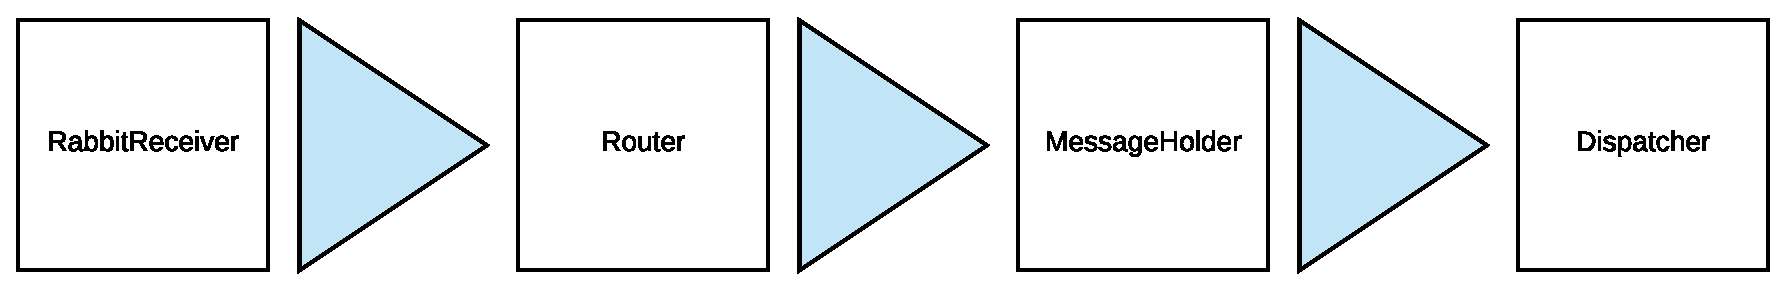
\includegraphics[width=\columnwidth]{images/solution/mw/inc/architect.eps}
  \caption{Incoming pipeline}
  \label{fig:mw-incoming}
\end{figure}

\begin{itemize}
  \item A RabbitReceiver is a process which receives messages from a single
    adjacent middleware node (or ``neighbor'') using RabbitMQ
  \item A Router compares the recipient field of the message with the
    identifier of the current node. If it is different, then it forwards the
    message to the next node along the path to the recipient
  \item A MessageHolder prevents messages to reach the dispatching point if a
    snapshot is happening. Then, when the snapshot ends, the messages will be
    forwarded again towards the Dispatcher
  \item A Dispatcher dispatches messages to a given service of the middleware
\end{itemize}

\begin{figure}[H]
  \centering
  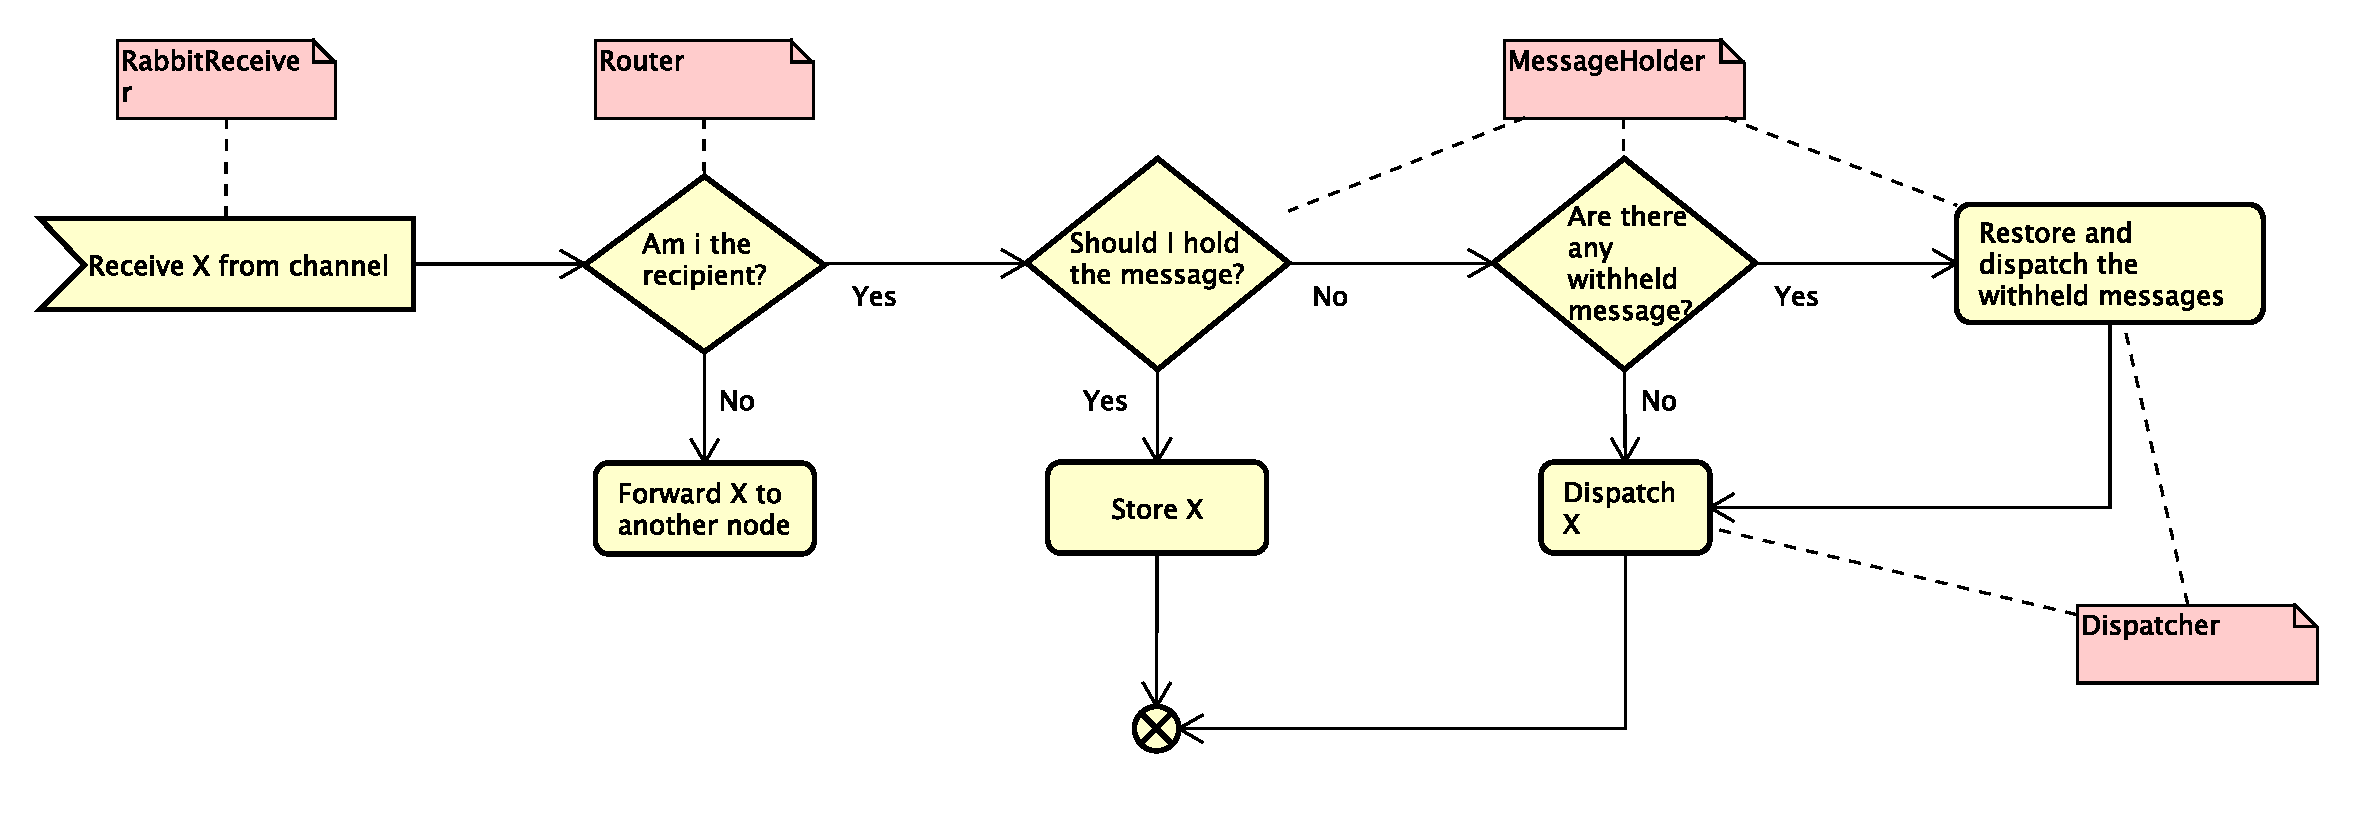
\includegraphics[width=\columnwidth]{images/solution/mw/inc/activity.eps}
  \caption{Activity diagram for Incoming pipeline}
  \label{fig:mw-incoming-activity}
\end{figure}

Thanks to the flexibility of GenStage, we can compose our pipelines by adding
an arbitrary number of elements at each stage of the pipeline. For instance,
there is one RabbitReceiver for each middleware neighbor plus one for loopback
communication: in this case, we just have to spawn as many RabbitReceivers as
needed and then make the Router subscribe to the events generated by them
(that is, the incoming messages).

\subsubsection{Interlayer service}

This component is responsible of the communication that is performed among
different layers, namely the one which it belongs (the \textbf{middleware}) and
another one who uses the middleware layer, that is the \textbf{application}
layer.

We show in figure \ref{fig:mw-interlayer} the architecture of this service and
then we will show in detail each module that composes this component.

\begin{figure}[H]
  \centering
  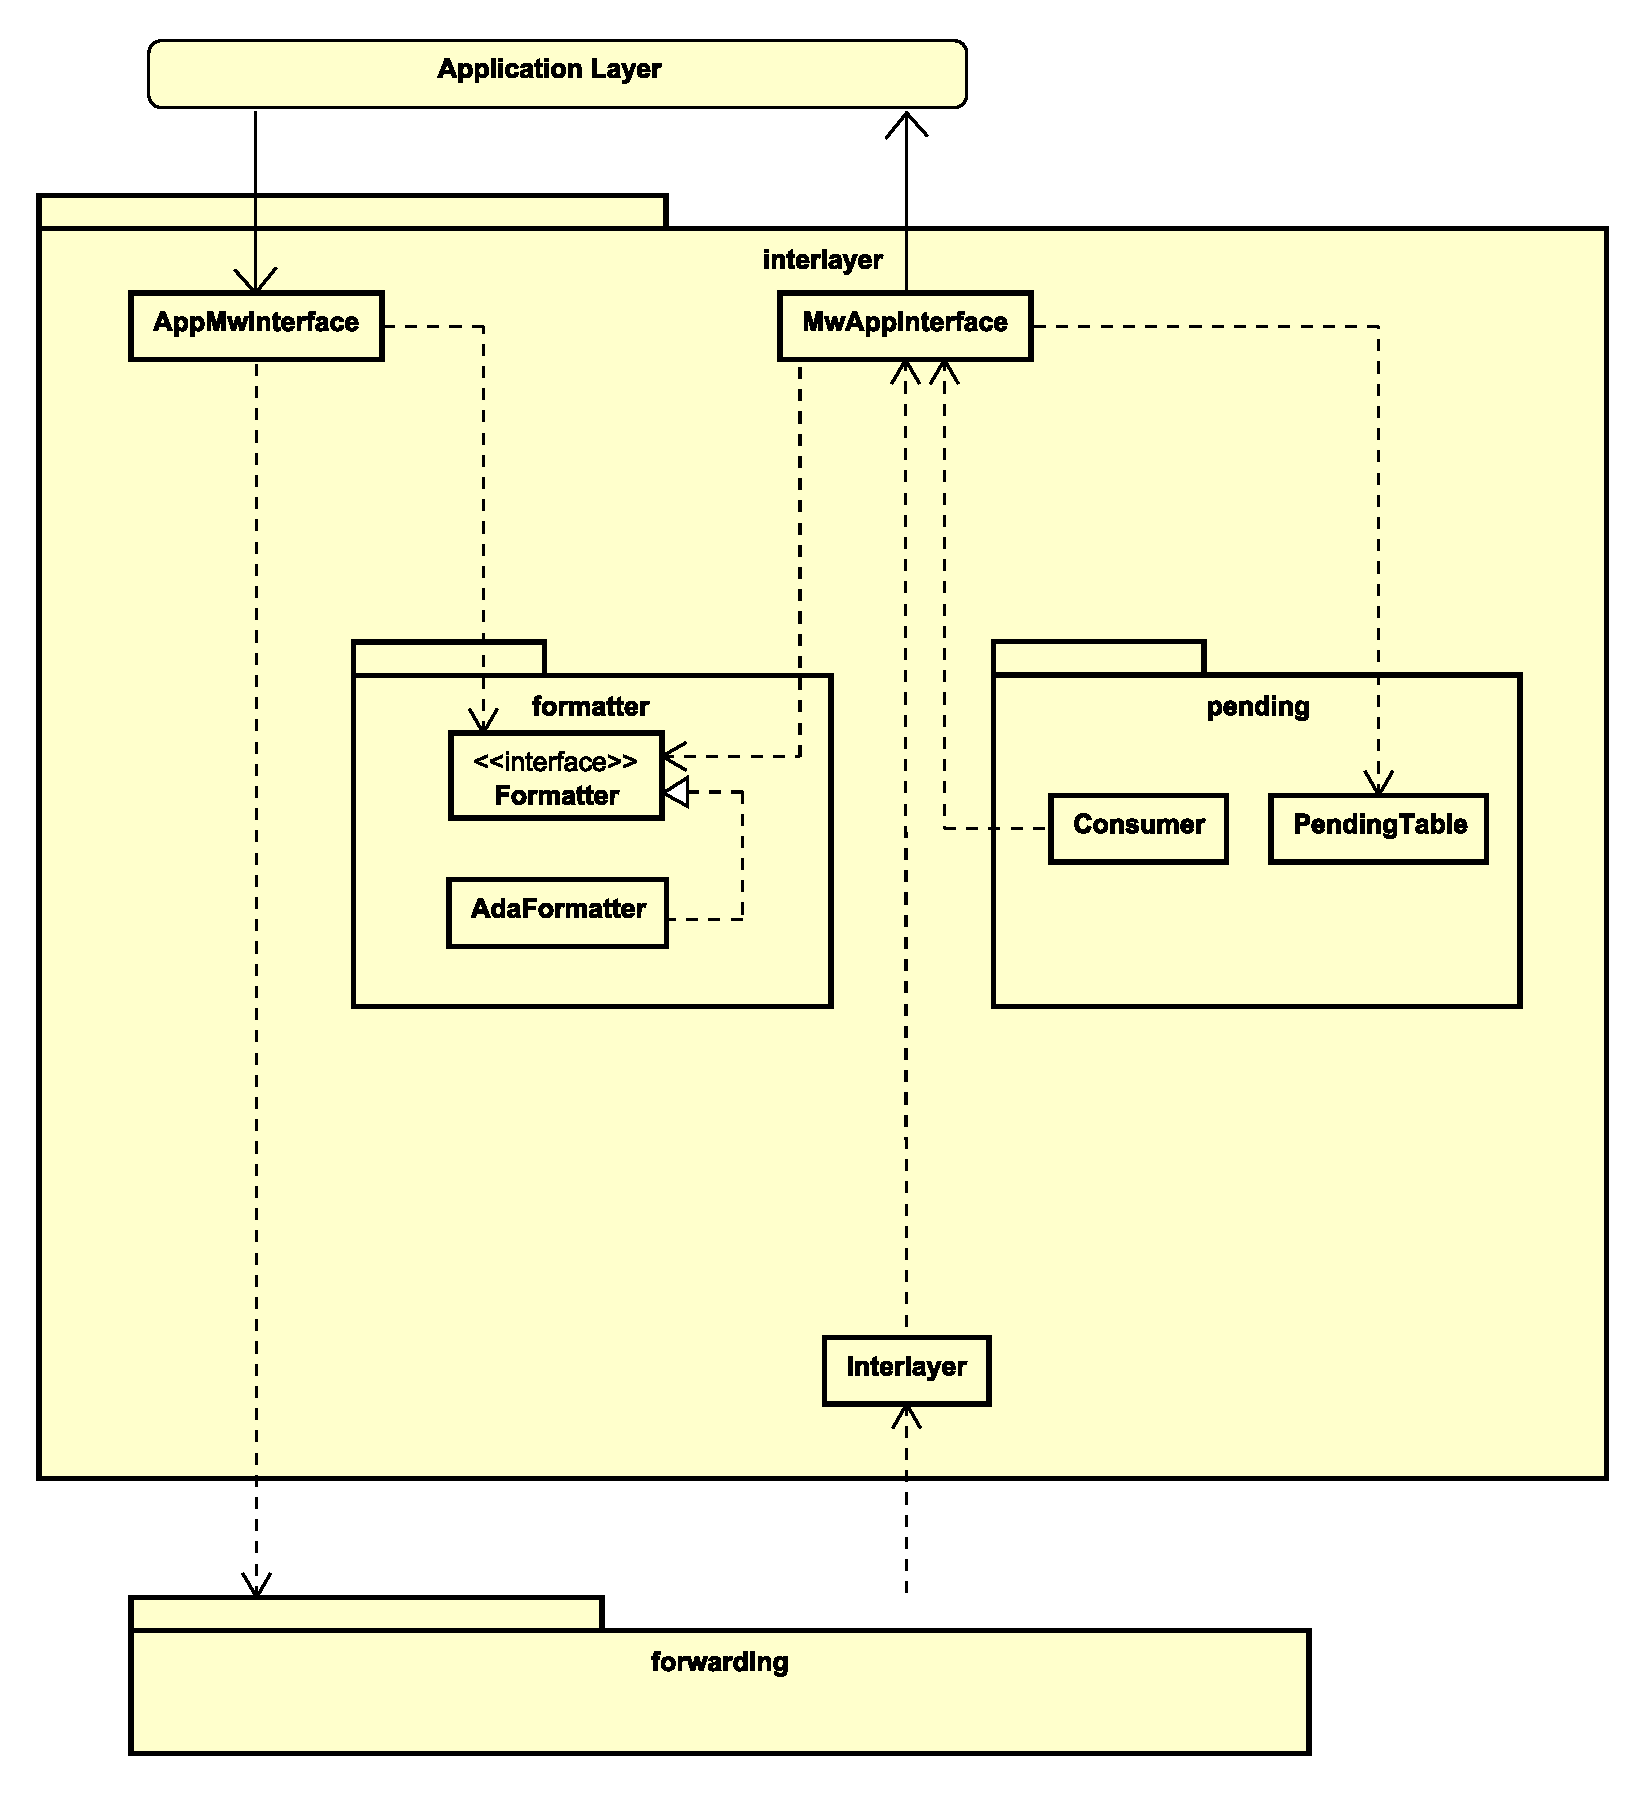
\includegraphics[width=\columnwidth]{images/solution/mw/interlayer.eps}
  \caption{Middleware's Interlayer service}
  \label{fig:mw-interlayer}
\end{figure} % TODO: needs update (Sequence usage comes from AppMwInterface)
             % TODO: how about removing AppDispatcher and Sequence?

% TODO: All class diagrams has to be added
\subsubsubsection{interlayer.Interlayer}
% TODO: Class diagram
\FloatBarrier
\begin{itemize}
  \item \textbf{Description} \\
    This module is the Fa\c cade of the Interlayer service. It is responsible
    to boot neatly and supervise all processes in Interlayer.
  \item \textbf{Attributes}
    \begin{itemize}
      \item \texttt{- sendPort: Int} \\
    TCP port messages will be directed to.
      \item \texttt{- listenPort: Int} \\
    TCP port messages will be received from.
    \end{itemize}
  \item \textbf{Operations}
  \begin{itemize}
    \item \texttt{+ start()} \\
    % TODO: check this out: Message will really be a String?
    Starts the Interlayer service.
    \item \texttt{+ handleMessage(message: String)} \\
    % TODO: check this out: Message will really be a String?
    Handles the reception of a message by ensuring it reaches the application
    layer.
  \end{itemize}
\end{itemize}

\subsubsubsection{interlayer.MwAppInterface}
% TODO: Class diagram
\FloatBarrier
\begin{itemize}
  \item \textbf{Description} \\
    Process that is responsible to deliver messages to the application layer.
  \item \textbf{Attributes}
    \begin{itemize}
      \item \texttt{- sendPort: Int} \\
    TCP port messages will be directed to.
      \item \texttt{- sendHost: String} \\
    Address messages will be directed to.
    \end{itemize}
  \item \textbf{Operations}
  \begin{itemize}
    \item \texttt{+ startLink(port: Int)} \\
    Starts the process and set \texttt{sendPort} to the value \texttt{port}.
    \item \texttt{+ toApplication(message: String)} \\
    % TODO: check this out: Message will really be a String?
    Sends a message to the application with reliable delivery.
    \item \texttt{+ send(message: String)} \\
    % TODO: check this out: Message will really be a String?
    Sends a message to the application with unreliable delivery.
  \end{itemize}
\end{itemize}

\subsubsubsection{interlayer.AppMwInterface}
% TODO: Class diagram
\FloatBarrier
\begin{itemize}
  \item \textbf{Description} \\
    Process that is responsible to receive messages from the application layer.
  \item \textbf{Attributes}
    \begin{itemize}
      \item \texttt{- listenPort: Int} \\
    TCP port messages will be received from.
    \end{itemize}
  \item \textbf{Operations}
  \begin{itemize}
    \item \texttt{+ start(port: Int)} \\
    Starts a server, setting \texttt{listenPort} to the value \texttt{port}.
    \item \texttt{- loopAcceptor(srv: PID)} \\
    Loops accepting requests as the server \texttt{srv}.
    \item \texttt{- serve(client: PID)} \\
    Handles the stream coming from the TCP connection of \texttt{client} by
    forwarding data towards to the Forwarding service.
  \end{itemize}
\end{itemize}

\subsubsubsection{interlayer.formatter.Formatter}
% TODO: Class diagram
\FloatBarrier
\begin{itemize}
  \item \textbf{Description} \\
    Interface for modules that translates messages to Elixir format from and
    to a (possibly) different one.
  \item \textbf{Operations}
  \begin{itemize}
    \item \texttt{+ format(msg: String)} \\
    Translates \texttt{msg} to the target format.
    \item \texttt{+ parse(msg: String)} \\
    Translates \texttt{msg} from the target format.
  \end{itemize}
\end{itemize}

\subsubsubsection{interlayer.formatter.AdaFormatter}
% TODO: Class diagram
\FloatBarrier
\begin{itemize}
  \item \textbf{Description} \\
    Module that implements the \texttt{interlayer.formatter.Formatter}
    interface for messages coming from an Ada application.
  \item \textbf{Attributes}
  \item \textbf{Operations}
  \begin{itemize}
    \item \texttt{+ format(data: String)} \\
    Format a message so that it can be received from an Ada application.
    \item \texttt{+ parse(data: String)} \\
    Parse a message that arrives from an Ada application.
  \end{itemize}
\end{itemize}

\subsubsubsection{interlayer.pending.PendingTable}
% TODO: Class diagram
\FloatBarrier
\begin{itemize}
  \item \textbf{Description} \\
    Process that keeps track of the messages that have not been sent yet to
    the application layer.
  \item \textbf{Attributes}
    \begin{itemize}
      \item \texttt{- pendingTable: Set<String>} \\
    Data structure in which pending messages are stored.
    \end{itemize}
  \item \textbf{Operations}
  \begin{itemize}
    \item \texttt{+ startLink()} \\
    Starts PendingTable process and retrieves pending messages from last
    execution (if there are some). \\
    Also starts an \texttt{interlayer.pending.Consumer}.
    \item \texttt{+ getnext()} \\
    If there are some pending messages, returns the first of them that has to
    be sent.
    \item \texttt{+ store(message: String)} \\
    Stores a message in the pending table.
    \item \texttt{+ remove(message: String)} \\
    Removes a message from the pending table.
  \end{itemize}
\end{itemize}

\subsubsubsection{interlayer.pending.Consumer}
% TODO: Class diagram
\FloatBarrier
\begin{itemize}
  \item \textbf{Description} \\
    Daemon worker that sequentially takes message from the pending table and
    tries to send them to the application layer.
  \item \textbf{Attributes}
  \item \textbf{Operations}
  \begin{itemize}
    \item \texttt{+ waitToConsume()} \\
    Waits for new messages to be available to be sent to the application layer.
  \end{itemize}
\end{itemize}

\subsubsection{Boot service}\label{sec:mw-boot-descr}

The Boot service is responsible of starting the system in a graceful fashion.
It does so by dividing the start phase into two subphases, namely the
\textbf{initialization} and the \textbf{boot} phase.

Initially, this service is in a \texttt{uninitialized} state, which means the
node has received neither a marker from a neighbor node to start the
initialization phase nor it has been acknowledged by the application layer that
its initialization is finished.

If the application layer tells the middleware that it's initialized, then the
Boot service will become \texttt{initialized}. If instead an initialization
marker arrives from a neighbor, the Boot service will stay in the
\texttt{uninitialized} state, waiting for the application layer to tell it's
initialized.
If the middleware receives another marker after having received the first one,
then it will reply immediately as it had finished its initalization phase.
Finally, when the Boot service has received all the initialization markers from
its neighbors and has been acknowledged by the application layer that it is
initialized, it will enter the \texttt{booting} state (and the \textbf{boot}
phase).

In the second phase this service waits for the boot marker (a middleware-layer
message which starts the boot of the system) to arrive. When it does, the Boot
service forwards the marker to all its neighbor and wait for all of them to
reply (i.e, for them to be booted).
When all the neighbors are booted, the application layer gets booted as
well and the Boot service sends a boot marker back.

The whole process is depicted in Figure \ref{fig:mw-boot}.

\begin{figure}[H]
  \centering
  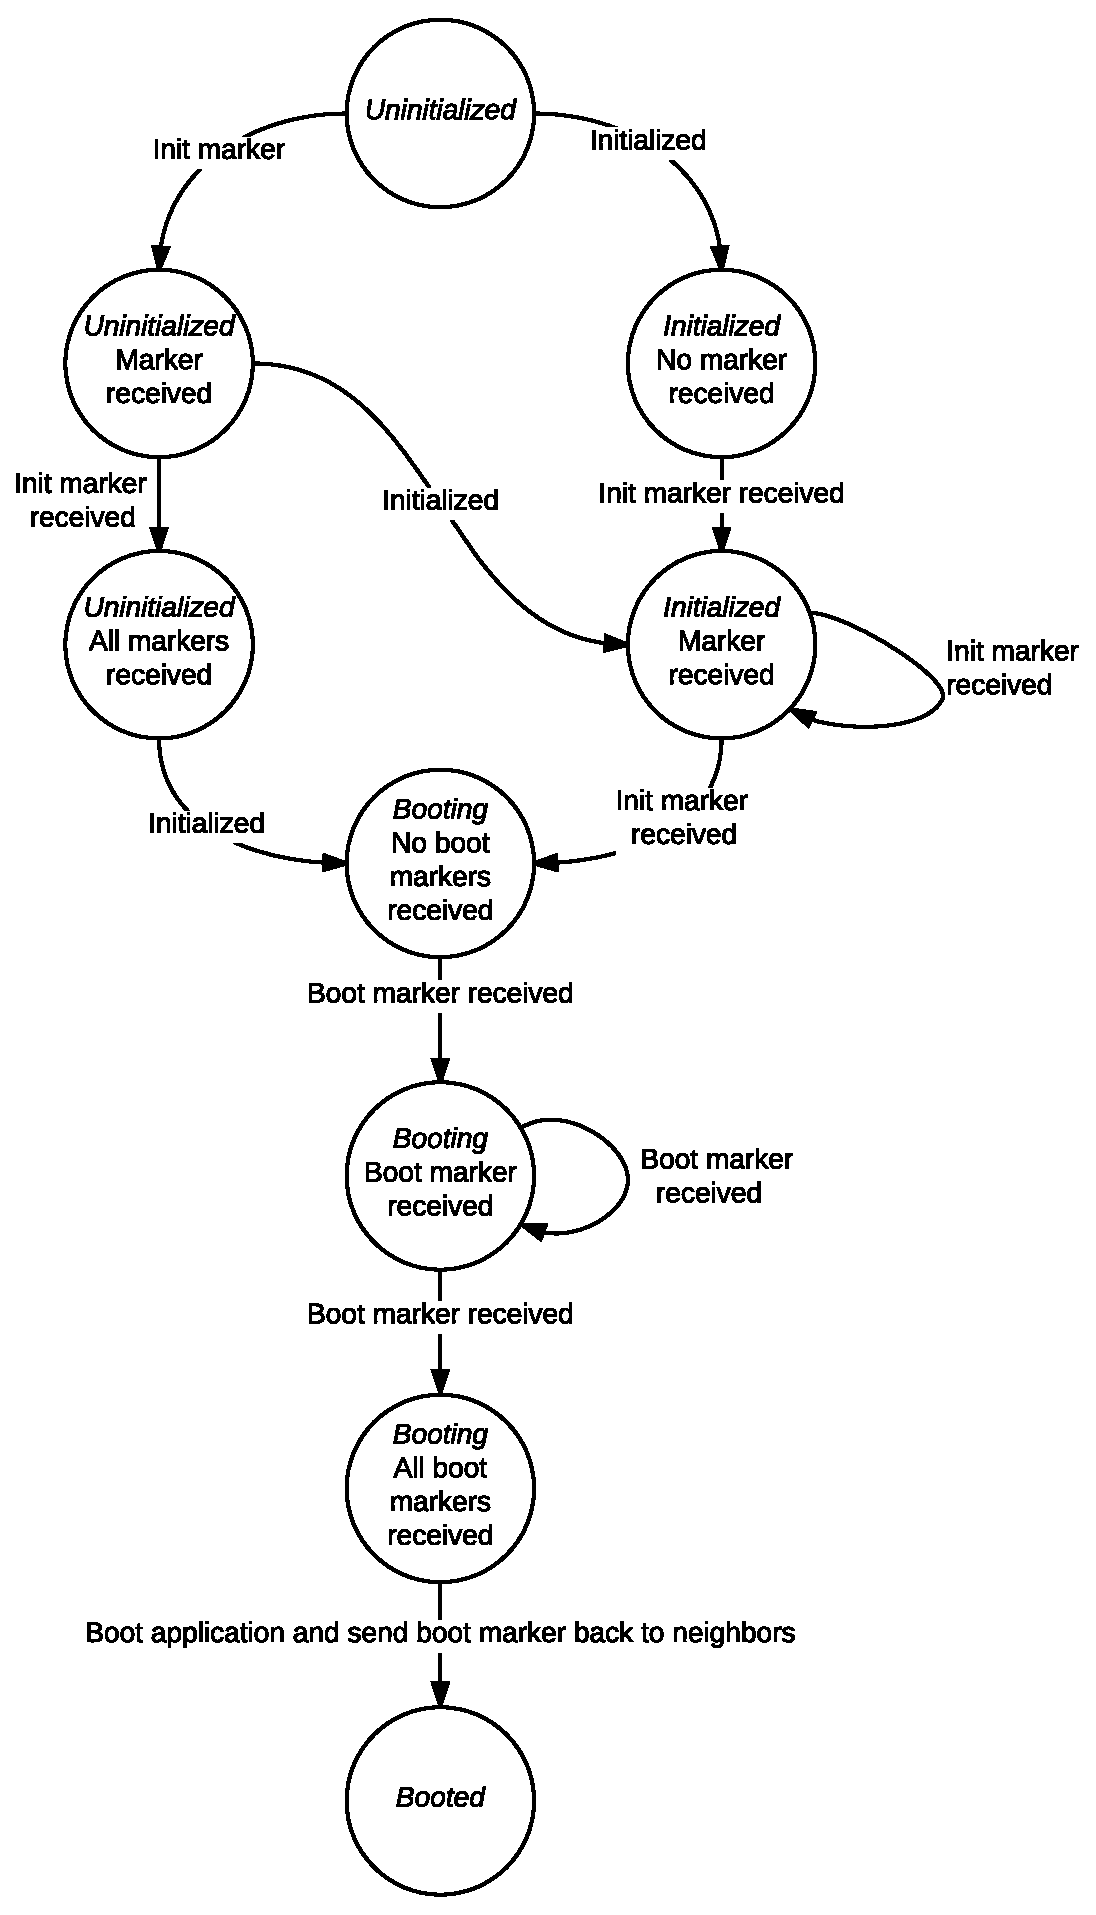
\includegraphics[width=.8\columnwidth]{images/solution/mw/boot.eps}
  \caption{Boot service: activity diagram}
  \label{fig:mw-boot}
\end{figure}

\subsubsection{Termination service}

\subsubsection{Snapshot service}

\subsubsection{Coordination service}

This component is responsible of the supervising the life-cycle of an
application run on our middleware, so our backend is able to operate
cohesively.

There are just two architectural units which compose this service:

\begin{enumerate}
\item a \texttt{Coordinator} initiates the boot process when requested and the
  termination process when the time limit for the application elapses;
\item \texttt{Monitor}s supervise the status of some services. In
  particular, we instantiated two monitor processes, one for the boot process
  and another one for the termination process. If a process $X$ does not end
  within a pre-configured time limit (we arbitrarily set 15 seconds for this
  parameter) after being started, the monitor issues again a request to
  perform $X$.
\end{enumerate}

\subsubsection{Persistence service}

This component is an adapter towards persistence and caching services.

More specifically, persistence is a collection of Redix wrappers. Redix is an
Elixir client for Redis, which handles all the network communication and
provides simple and convenient API to access Redis services.
Therefore, we just have to specify some of the CRUD operations for a certain
data structure we are interested in -- it could be a map (e.g., for pending
requests, so that we are able to correlate an id to a given request) or a
queue (e.g., pending unsent messages directed to the application layer).

However, we stress the fact that even if Persistence service uses Redis, it
could have used anything else without changing its API (the persistence
technology we employed is completely transparent to the other middleware
services).

